\documentclass[journal ]{new-aiaa}
%\documentclass[conf]{new-aiaa} for conference papers
\usepackage[utf8]{inputenc}
\usepackage{textcomp}

\usepackage{graphicx}
\usepackage{amsmath}
\usepackage[version=4]{mhchem}
\usepackage{siunitx}
\usepackage{longtable,tabularx}
\setlength\LTleft{0pt} 

\title{A Comprehensive Review on the Development of Computational Frameworks for Spacecraft Fragmentation and Orbital Debris Population Dynamics}

\author{Juan F Puerta-Ibarra \footnote{juanf.puerta@udea.edu.co (J.F.P.-I.)}}
\affil{Research Group in Efficient Energy Management (GIMEL), Departamento de Ingeniería Eléctrica, Universidad de Antioquia, Calle 67 No. 56-108, Medellin 050010, Colombia}
\author{Nicolás Muñoz-Galeano\footnote{nicolas.munoz@udea.edu (N.M.-G.)}}
\affil{Research Group in Efficient Energy Management (GIMEL), Departamento de Ingeniería Eléctrica, Universidad de Antioquia, Calle 67 No. 56-108, Medellin 050010, Colombia}

\begin{document}

\maketitle

\begin{abstract}
The increasing prevalence of spacecraft fragmentation and the resultant growth of orbital debris present significant challenges to the sustainability of space operations. This review comprehensively examines the evolution of computational frameworks developed to model spacecraft fragmentation and the dynamics of orbital debris populations. It highlights key methodologies, including empirical models, semi-empirical approaches, and advanced simulation techniques, that have emerged over the past few decades. The paper discusses the implications of fragmentation events, the Kessler Syndrome, and the importance of accurate debris population predictions for collision risk assessment and mitigation strategies. Furthermore, it emphasizes the need for innovative approaches that integrate insights from fragmentation models with advanced computational techniques, such as symplectic integrators, to enhance the accuracy and efficiency of debris tracking and management. By synthesizing recent research trends and identifying gaps in the current literature, this review aims to inform future research directions and contribute to the development of effective strategies for ensuring the long-term sustainability of the orbital environment.
\end{abstract}

\textbf{Keywords:} Spacecraft Fragmentation, Orbital Debris, Computational Frameworks, Kessler Syndrome, Collision Risk Assessment, Debris Mitigation, Modeling and Simulation, Space Environment, Fragmentation Events, Space Traffic Management


\section{Introduction}
\lettrine{F}ragmentation of space debris is a critical issue in the context of increasing space activities and the sustainability of the orbital environment. Since the dawn of the space age, the number of artificial objects in orbit has grown significantly, with estimates indicating over 31,000 objects larger than 10 cm and approximately 500,000 objects larger than 1 cm currently in low Earth orbit (LEO) ~\cite{petit_impact_2016}. Fragmentation events, which can occur due to collisions, explosions, or structural failures, contribute substantially to the debris population. For example, intentional destruction of satellites and accidental collisions have been responsible for generating a significant portion of the debris, with catastrophic events leading to the creation of thousands of fragments ~\cite{pardini_review_2014}. The Kessler syndrome, a scenario in which the density of objects in LEO becomes so high that collisions become inevitable, underscores the urgency of addressing fragmentation and its implications for operational spacecraft ~\cite{petit_impact_2016}.

The dynamics of space debris fragmentation are complex and influenced by various factors, including the physical properties of the objects involved, the nature of the fragmentation event, and the orbital environment. Fragmentation models, such as the NASA Standard Breakup Model, provide a framework for understanding the size and velocity distributions of debris generated during such events. These models have evolved over the years, incorporating data from ground tests and on-orbit events to improve their predictive capabilities ~\cite{johnson_nasas_2001}. The challenge lies in accurately modelling the fragmentation process, as the resulting debris can vary widely in size and behaviour, complicating the assessment of collision risks and the long-term evolution of the debris environment ~\cite{mains_impact_2021}.

Multibody orbit propagation is essential for analyzing the trajectories of both intact satellites and fragments resulting from fragmentation events. Traditional methods often focus on larger debris objects, neglecting the significant contribution of smaller fragments to collision probabilities ~\cite{letizia_collision_2016}. Recent advancements in modeling techniques, such as the Particle-In-a-Box (PIB) approach, allow for a more comprehensive analysis of the debris population by treating fragments as a continuous density rather than individual objects ~\cite{giudici_density-based_2024}. This method enhances computational efficiency and enables the assessment of the cumulative effects of small debris on operational spacecraft. Furthermore, the integration of atmospheric models and space weather data into orbit propagation studies is crucial for understanding the long-term dynamics of debris clouds and their potential impact on space operations.

The interplay between space debris fragmentation and multibody orbit propagation presents significant challenges to the sustainability of the space environment. As the number of objects in orbit continues to rise, understanding the mechanisms of fragmentation and developing robust models for predicting debris behaviour are essential for mitigating risks to operational spacecraft and ensuring the long-term viability of space activities. Ongoing research and advancements in modelling techniques will be vital in addressing these challenges and informing effective debris mitigation strategies.

To effectively navigate this complex and evolving field, bibliometrics serve as crucial tools for identifying trends, influential publications, and key authors. By analyzing citation patterns, publication frequencies, and collaboration networks, bibliometric studies can shed light on research dynamics and highlight significant contributions to the body of knowledge surrounding space debris and orbit propagation. Leveraging tools such as VOSviewer, Litmaps, and PyBibX enables researchers to visualize academic landscapes, pinpoint clusters of related work, and identify pivotal papers and thought leaders. This analysis fosters a deeper understanding of the current state of the field and supports the development of innovative solutions for space sustainability.

\subsection{Literature review purpose.}

The purpose of the review is to uncover critical insights through bibliometric analysis, including gaps in the literature, influential papers, and emerging themes in the field of space debris fragmentation and multibody orbit propagation. By systematically mapping the academic landscape, the review aims to inform future research directions and enhance understanding of the current state of knowledge in this area. A comprehensive survey of existing fragmentation and debris models is conducted, focusing on their methodologies, strengths, and limitations in the context of space debris management. This includes an examination of well-established models such as the NASA Standard Breakup Model (SBM) and other empirical and semi-empirical approaches that characterize the generation and evolution of debris clouds resulting from fragmentation events. The review will also explore the potential of symplectic orbit propagators in n-body propagation scenarios, emphasizing their advantages in preserving the Hamiltonian structure of dynamical systems and their effectiveness in long-term simulations of orbital mechanics ~\cite{hubaux_symplectic_2012}. By integrating insights from fragmentation models with advanced symplectic methods, the review aims to identify opportunities for enhancing the accuracy and efficiency of debris population predictions and collision risk assessments in complex orbital environments.

This exploration is particularly relevant given the increasing complexity of space operations and the growing population of space debris, necessitating robust models that can accurately simulate the interactions and evolution of multiple debris objects over time. The review will highlight the need for innovative approaches that combine the strengths of fragmentation modelling with the computational efficiency of symplectic propagators ~\cite{cintio_symplectic_2017}, ultimately contributing to improved strategies for debris mitigation and space traffic management.

\section{Methodology}

To provide a comprehensive review of spacecraft fragmentation and orbital debris, a multistage search strategy was developed using several databases and online tools, such as Scopus, Google Scholar and Litmaps. Scopus, which is one of the largest abstract and citation databases for peer-reviewed literature, was intensively selected for its extensive coverage of the aerospace and engineering domains. A series of four initially targeted searches were conducted, each focusing on a specific aspect related to orbital debris and spacecraft fragmentation, as well as relevant computational methods for orbital analysis.

These proposed queries were: \textit{spacecraft fragmentation orbital debris}, \textit{0space debris orbit propagator}, \textit{symplectic orbit integrators} and \textit{n-body rebound}. Each search query addressed a specific subtopic of interest within the broader theme of spacecraft fragmentation and orbital debris dynamics.

\begin{itemize}
    \item \textit{Spacecraft Fragmentation Orbital Debris:} This first query is the main search of this review, focused on identifying the literature that discusses the mechanisms and consequences of spacecraft fragmentation and the subsequent creation of orbital debris. The goal was to collect information about the formation, characteristics, and hazards of debris generated by fragmentation events. 149 papers were found.
    \item \textit{Space Debris Orbit Propagator:} The second query aimed to retrieve papers related to the modeling and simulation of orbital debris trajectories, specifically focusing on orbit propagators that predict the movement of debris over time. This is critical to understanding how debris evolves in Earth’s orbit and poses risks to operational spacecraft. 101 papers were found.
    \item \textit{Symplectic Orbit Integrators:} This search was designed to identify papers that examine the use of symplectic integration methods for long-term orbit propagation. Symplectic integrators are known for their ability to maintain the stability of orbit calculations over extended periods, making them essential in debris modeling and collision risk assessments. 183 papers were found.
    \item \textit{N-body REBOUND:} The fourth query focused on the use of n-body simulation techniques and the REBOUND code to model the interactions between multiple objects in space. This technique is particularly useful for analyzing complex interactions within orbital debris clouds and assessing potential collision scenarios. 31 papers were found.
\end{itemize}

A combination of these four search queries ensured that the resulting set of papers covered both theoretical and practical aspects of spacecraft fragmentation, orbital debris dynamics, and advanced simulation methods. After conducting the searches, a total of 464 papers were identified as relevant and selected for further analysis. The use of Litmaps added more research papers to the final number due to its capacity to connect the actual papers to cited ones online. The inclusion criteria for the articles were based on their relevance to the topic, publication in peer-reviewed journals or conferences, and availability of full-text access. Papers older than 30 years or those with minimal citations were excluded unless they contributed to foundational theories or models still referenced today.

\subsection{VOSviewer and PyBibX Analysis}
To analyze the selected articles and identify key trends, the VOSviewer and PyBibX tools were used. VOSviewer is a widely used software tool designed for creating and visualizing bibliometric networks. It is especially useful in generating network maps based on data from bibliographic databases such as Scopus and Web of Science. These networks can represent relationships between various entities, including co-authorship networks, citation networks, keyword co-occurrence networks, and bibliographic coupling.VOSviewer was used to perform bibliometric analyses such as citation mapping, co-occurrence keyword networks, and bibliographic coupling of organizations. This allowed visualization of relationships between papers, keywords, and contributing institutions, providing insight into the most influential authors and trends in the field.

In addition, PyBibX is a Python-based tool that is used for advanced bibliometric analysis. While VOSviewer specializes in visualization, PyBibX focuses more on providing detailed bibliometric metrics and analysis of citation data. It can be used to extract and analyze bibliometric data from sources like Scopus and Web of Science as well, and it allows for flexible, customized analysis using Python.

The citation analysis revealed the most frequently cited papers, highlighting seminal works that have shaped the current understanding of spacecraft fragmentation and orbital debris. Keyword cooccurrence analysis enabled the identification of the most prominent research themes, including orbital debris mitigation, collision risk assessment, and debris propagation modeling. Additionally, bibliographic coupling allowed for the identification of key institutions, such as NASA, the European Space Agency (ESA), and leading universities that have contributed extensively to the body of knowledge on orbital debris.

Through this combination of Scopus searches and advanced bibliometric tools, the review was able to provide a detailed synthesis of the current state of research and identify areas where further investigation is needed.

\subsection{Litmaps and DocAnalyzer.}

Litmaps and DocAnalyzer are valuable tools for researchers conducting literature reviews, particularly in complex and evolving fields such as aerospace engineering. Each tool offers unique capabilities that can enhance the process of gathering, organizing, and analyzing academic research, making it easier to identify trends, explore relationships between studies, and uncover research gaps.

\subsubsection{Litmaps.}

Litmaps serves as a dynamic platform for visualizing connections among academic papers through citation networks, which allows researchers to track how studies are interrelated. By mapping out these networks, Litmaps reveals how new research builds upon previous work or offers alternative perspectives. This feature is invaluable in fields such as orbital debris modeling, where understanding the development and connections among different models and techniques can significantly impact the research direction. Additionally, Litmaps allows researchers to set up alerts for specific topics or keywords, notifying them when relevant new studies or preprints are published. This enables users to stay up to date with the latest developments, making it easier to incorporate fresh insights into their literature review and ensure that they are referencing up-to-date sources. By following these citation trails and alerts, researchers can more easily identify seminal papers and observe how fields are evolving.

\subsubsection{DocAnalyzer.}

DocAnalyzer complements Litmaps by offering powerful text analysis and summarization capabilities, making it easier for researchers to distill key insights from large datasets of academic papers. Instead of reading each paper in full, DocAnalyzer extracts essential themes, keywords, and summaries, allowing a quick understanding of the core ideas of a paper. This is particularly beneficial when dealing with high volumes of research on niche topics such as fragmentation models or symplectic orbit propagation techniques. DocAnalyzer also facilitates the identification of patterns and common themes within a field by recognizing frequently occurring terms or concepts. This helps researchers categorize various approaches or methodologies, for example, differentiating between analytical, empirical, and numerical methods in debris modeling, or pinpointing major challenges in symplectic methods.

Moreover, DocAnalyzer offers contextual analysis by mapping relationships between concepts across multiple documents. This feature provides insight into how different studies address similar issues, such as the trade-offs between computational efficiency and accuracy in orbit propagators. Finally, by extracting key terms and concepts, DocAnalyzer aids in synthesizing information across papers, helping researchers structure their literature reviews more cohesively and uniformly, especially in fields where terminology can vary widely.

Together, Litmaps and DocAnalyzer provide a comprehensive toolkit for literature reviews. Litmaps delivers a broad overview of research connections and evolution, while DocAnalyzer enables detailed document analysis and synthesis. This combination supports the creation of literature reviews that are both wide-ranging and analytically deep, helping researchers produce well-organized and insightful reviews on complex topics.

\section{Analysis Results}

This section aims to elucidate the effectiveness of different modeling approaches in predicting debris generation, tracking the evolution of debris clouds, and assessing the associated risks to operational spacecraft. By analyzing the results obtained from established models, such as the NASA Standard Breakup Model and newer methodologies, this section highlights the advances made in the field and identifies key trends that inform future research directions in debris mitigation and management strategies. Based on the methodology described in the last section, these are the results.

\subsection{Author Citation}

\begin{figure}[hbt!]
    \centering
    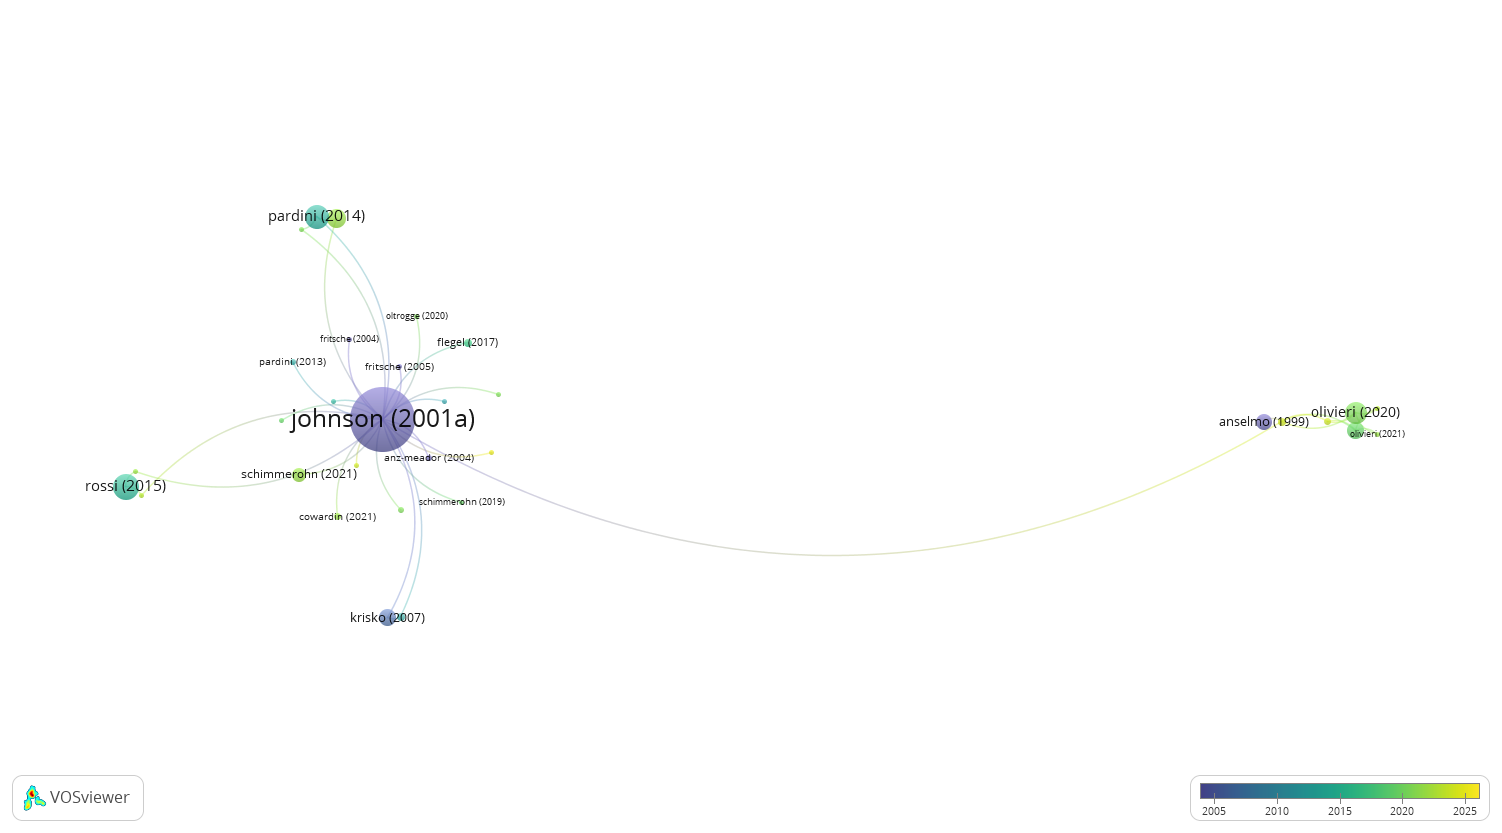
\includegraphics[width=\textwidth]{sfod_citation.png}
    \caption{Visualization of the citation network generated by VOSviewer, based on a bibliometric analysis of papers related to spacecraft fragmentation and orbital debris.}
    \label{fig:sfod_citation}
\end{figure}

\label{fig:sfod_citation} is a visualization of the citation network generated by VOSviewer, based on a bibliometric analysis of papers related to spacecraft fragmentation and orbital debris, using the data extracted from Scopus. The image provides several insights based on the relationships between papers and the way they cite each other. Each circle represents a paper, and the size of each node indicates its relevance or importance in the network based on the number of citations it has received. A larger node means a paper that has been cited frequently in other works. The lines connecting the nodes represent the citation links between the papers. The more connected a node is, the more it has influenced other works in the domain.

\textbf{Clusters and Groups.}

\begin{itemize}
    \item Johnson (2001a) ~\cite{johnson_nasas_2001} is clearly a central and highly influential paper in this field. Its central position and large node size indicate that many subsequent works refer to it. Several other papers, such as Krisko (2007) ~\cite{krisko_predicted_2007} and Pardini (2014) ~\cite{pardini_review_2014}, are clustered around Johnson's work, suggesting that they are closely related or have built upon its findings.
    \item Rossi (2015)~\cite{rossi_criticality_2015} and Olivieri (2020) ~\cite{olivieri_investigation_2021} are also notable, although somewhat isolated compared to Johnson's paper, but still showing relevance in the field.
    \item The connection between Johnson (2001a) and Krisko (2007) likely suggests that these papers are foundational in the field of spacecraft fragmentation and orbital debris, and they have provided significant contributions that are built upon by others.
\end{itemize}

\textbf{Color Gradient (Timeline).}

\begin{itemize}
    \item The coloring of the nodes represents the publication timeline of these works. Papers in blue and purple are from earlier years (likely 1999-2005), while yellow and green represent newer papers published in more recent years (closer to 2020-2025).
    \item Johnson (2001a) is an older but highly cited work, which has spawned numerous follow-up studies over the years, indicated by connections to papers in green and yellow.
    \item Olivieri (2020) and its connected papers in green and yellow highlight recent developments in the domain of space debris fragmentation, indicating active research interest.
\end{itemize}

\textbf{Notable Connections.}

\begin{itemize}
    \item The presence of Rossi (2015) and its connection to the network indicates a significant contribution, though it may be on a different subtopic compared to the core cluster around Johnson (2001a).
    \item The network on the right, around Olivieri (2020), suggests newer and potentially more innovative research trends, especially in 2020 and beyond, signaling emerging research areas in the field.
\end{itemize}

\textbf{Analysis.}
\begin{itemize}
    \item Johnson (2001a) remains a seminal work in spacecraft fragmentation and orbital debris, influencing multiple subsequent papers and studies. It likely presents foundational theories, models, or data that have shaped much of the current understanding in the field.
    \item Rossi (2015) and Olivieri (2020) represent important contributions, particularly in more recent developments. However, they appear slightly isolated, suggesting that these papers might be focusing on different or novel approaches that are less directly connected to the foundational models of the earlier papers.
    \item The density of connections between nodes, particularly around Johnson (2001a), indicates that much of the research on space debris fragmentation is interrelated, with researchers building upon previous works to expand the body of knowledge.
    \item The timeline of publications shows that research in this field is ongoing, with new insights and models being published through 2020-2025, indicating that the problem of orbital debris is an active and evolving area of study.
\end{itemize}

\subsection{Co-occurrence keywords.}

\begin{figure}[hbt!]
\centering
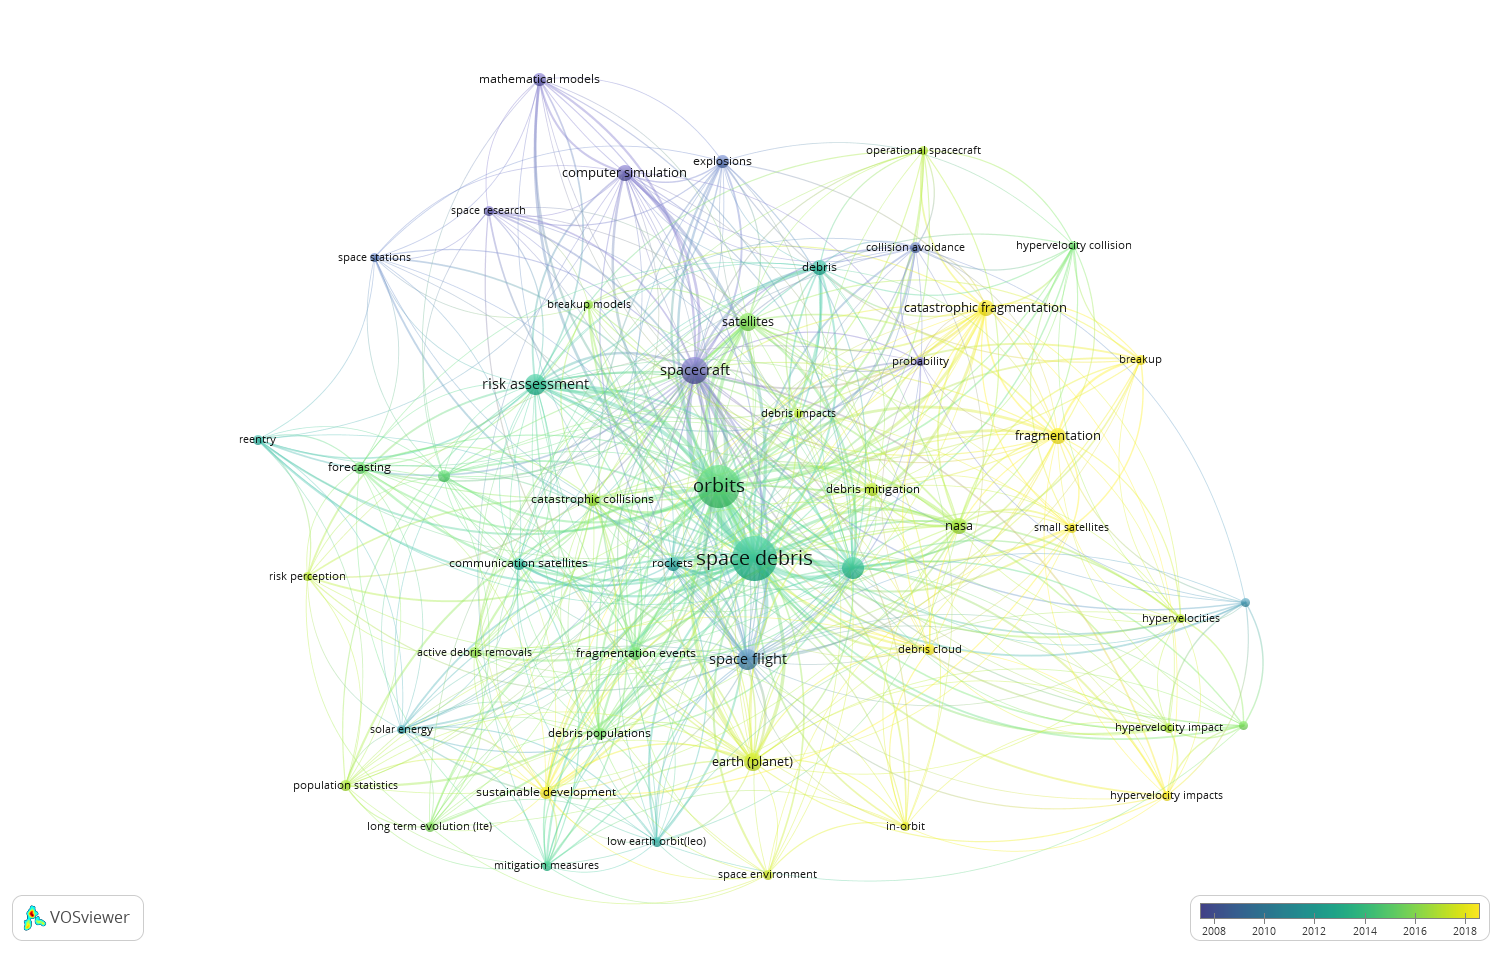
\includegraphics[width=\textwidth]{sfod_coocurrence_keywords.png}
\caption{Co-occurrence network of keywords related to spacecraft fragmentation and orbital debris.}
\end{figure}

This image represents a co-occurrence network of keywords related to spacecraft fragmentation and orbital debris, based on the bibliometric analysis of publications from Scopus. Each node represents a keyword, and the connections between them show how frequently these keywords appear together in academic papers.

\textbf{Central Cluster (green/yellow).}

\begin{itemize}
    \item Core keywords include "space debris", "orbits", and "space flight". These keywords are at the heart of the research and are highly related to a wide range of other topics.
    \item The focus on space debris indicates that this is the primary issue being addressed in this research area. The term is connected to several adjacent topics like debris mitigation, fragmentation, debris clouds, and operational spacecraft.
    \item NASA appears prominently, suggesting a strong involvement of the agency in both research and mitigation efforts related to space debris.
\end{itemize}

\textbf{Top-Left Cluster (purple/blue).}

\begin{itemize}
    \item This cluster includes keywords such as "mathematical models", "computer simulation", and "space research".
    \item These terms are older and focus on the modeling and simulation aspects of space debris and fragmentation, which form the basis for theoretical understanding.
    \item Mathematical models are critical for simulating the behavior of space debris and predicting collision risks, forming the backbone of fragmentation analysis and orbital debris studies.
\end{itemize}

\textbf{Right Side Cluster (green/yellow).}

\begin{itemize}
    \item This cluster focuses on more technical and operational aspects of fragmentation, including terms such as "fragmentation", "catastrophic fragmentation", and "hypervelocity impacts".
    \item This suggests a more recent interest in high-speed collisions and the effects of hypervelocity on debris, which are important in understanding how fragmentation events generate more debris in space.
    \item The terms breakup and catastrophic fragmentation indicate that research has shifted toward studying the severe consequences of fragmentation events and their impact on space missions.
\end{itemize}

\textbf{Bottom Cluster (green/yellow).}

\begin{itemize}
    \item Keywords such as "sustainable development", "low earth orbit" (LEO), "mitigation measures", and "active debris removal" show the growing importance of sustainability in space operations.
    \item The emphasis on mitigation suggests that researchers are focusing on solutions to the space debris problem, such as debris removal technologies and disposal strategies.
    \item Low Earth Orbit (LEO) is of particular concern because it is a densely populated orbital region, and many mitigation efforts focus on keeping this region clear of hazardous debris.
\end{itemize}

\textbf{Top-Right Cluster (yellow/green).}

\begin{itemize}
    \item This small, more recent cluster revolves around specific topics like "hypervelocity collisions", "debris impacts", and "collision avoidance".
    \item These topics are critical for modern-day spacecraft operations, as the risk of collisions with debris is one of the main operational challenges in space.
\end{itemize}

\subsection{Coupling organizations.}

\begin{figure}[hbt!]
\centering
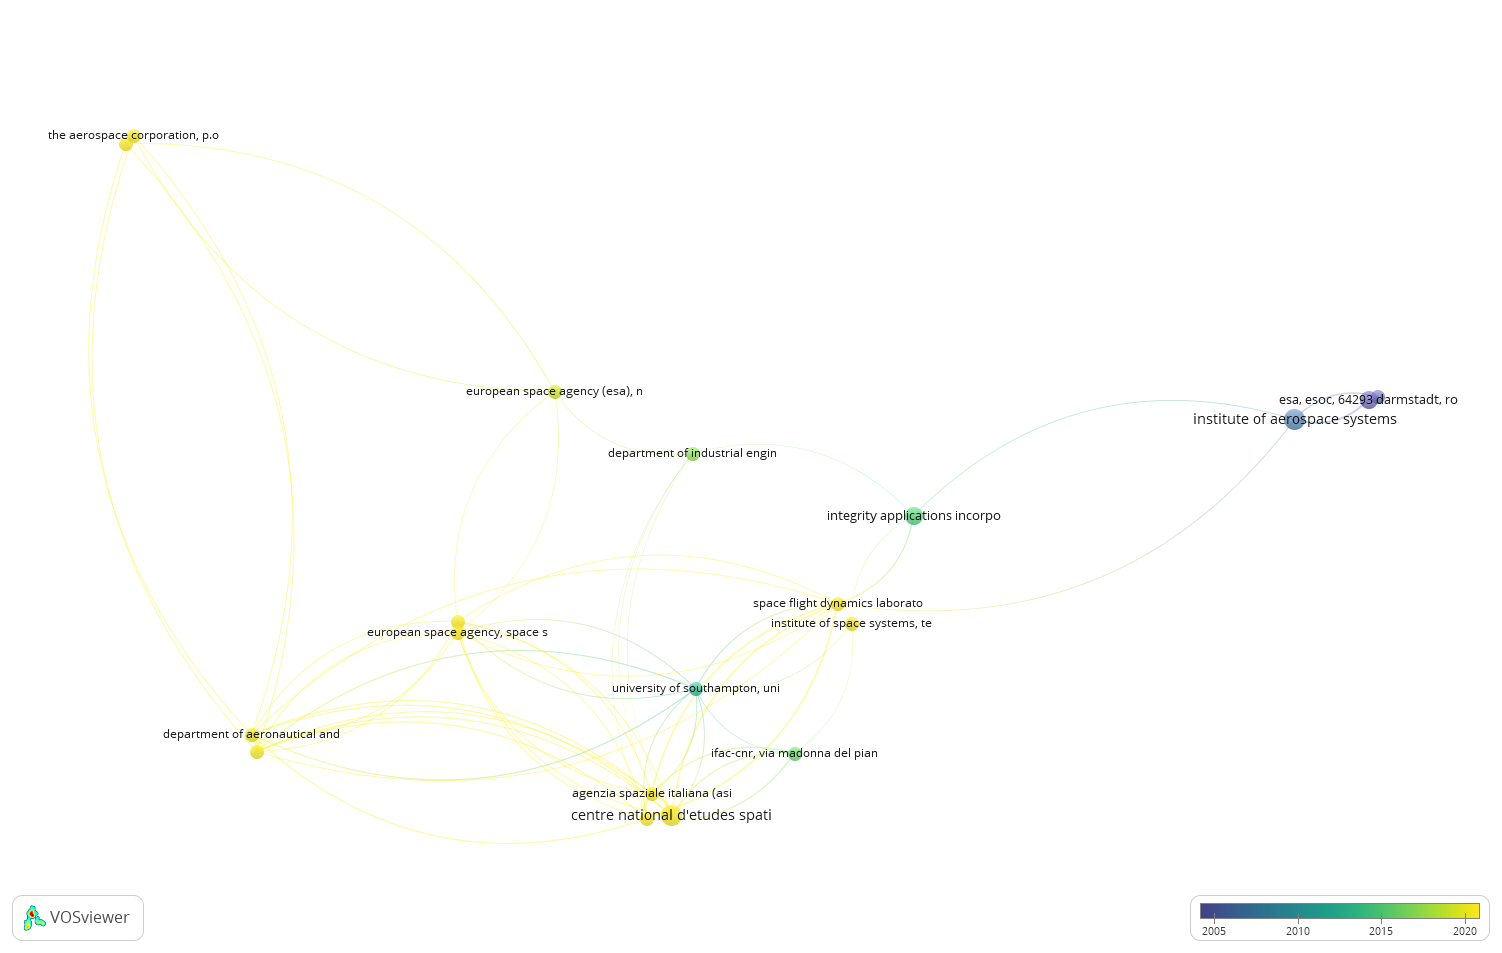
\includegraphics[width=\textwidth]{sfod_b-coupling_organizations.png}
\caption{Visualization of the bibliometric analysis results, showing the relationships between organizations.}
\end{figure}

 This visualization represents bibliographic coupling of organizations in the field of spacecraft fragmentation and orbital debris. Bibliographic coupling occurs when two organizations cite the same third-party paper, indicating that they are likely researching similar topics.

\textbf{Left Side (Yellow/Green Cluster).}

\begin{itemize}
    \item Organizations like The Aerospace Corporation and European Space Agency (ESA) dominate this side of the graph.
    \item The ESA appears multiple times, which likely indicates that its sub-organizations (e.g., European Space Agency, Space S, European Space Agency (ESA), etc.) are actively collaborating or working on distinct but related projects.
    \item This cluster focuses on more recent research (yellow nodes), with strong involvement from space agencies such as ESA and Agenzia Spaziale Italiana (ASI). These agencies are at the forefront of recent developments in spacecraft fragmentation and debris management.
\end{itemize}

\textbf{Right Side (Blue/Green Cluster).}

\begin{itemize}
    \item ESA's European Space Operations Centre (ESOC) of ESA in Darmstadt, together with the Institute of Aerospace Systems, form an important node in this region. These organizations are linked with more historical research (blue nodes), and are still relevant but with less recent output compared to the yellow cluster.
    \item ESOC seems to be a key player in early works on spacecraft fragmentation and orbital debris, likely focusing on space operations and debris monitoring.
\end{itemize}

\textbf{Middle Cluster (Mixed Timeline).}

\begin{itemize}
    \item University of Southampton, Space Flight Dynamics Laboratory, IFAC-CNR, and other institutions make up this middle ground, with green nodes. These institutions have more balanced contributions over time.
    \item University of Southampton and other academic institutions appear to play a bridging role between highly specialized space agencies and technical laboratories, as they collaborate with both.
\end{itemize}

\textbf{Analysis.}
\begin{itemize}
    \item Core Institutions: The European Space Agency (ESA) is a central node, with many of its sub-organizations actively involved in research related to space debris. Aerospace Corporation and European institutions like CNES (Centre National d'Études Spatiales) and ASI are also key players. Their strong coupling indicates that these institutions are leading the charge in studying spacecraft fragmentation and mitigating orbital debris.
    \item Recent and Historical Contributions.
    \begin{itemize}
        \item Organizations with yellow nodes represent more recent contributors to the research, including ESA and its associated projects.
        \item Blue and green nodes represent historically significant contributors, like ESOC, who have been publishing since earlier years but are still relevant.
    \end{itemize}
    \item Space Agencies and Academia: There seems to be a strong collaboration between space agencies (ESA, ASI, CNES) and academic institutions (University of Southampton, Institute of Aerospace Systems), suggesting a synergistic relationship where space missions and practical operations are informed by academic research and vice versa.
\end{itemize}

\textbf{Insights and Implications.}
\begin{itemize}
    \item ESA's Role: The prominence of ESA and its multiple sub-organizations indicates its leadership in space debris management research. Their coupling with other institutions suggests that they are working closely with both European and international partners.
    \item Inter-agency and Inter-institutional Collaboration: The network highlights inter-agency cooperation, as seen between ESA, Aerospace Corporation, CNES, and ASI. Such collaboration is vital for addressing global challenges such as space debris.
    \item Shifting Focus Over Time: The color gradient suggests a transition in the focus of research. Earlier work (blue nodes) might have laid the theoretical foundations, while more recent publications (yellow nodes) likely focus on applied solutions and mitigation techniques.
    \item Geographical Diversity: The institutions in this network span different countries, indicating the international nature of space debris research. This is a field that benefits from global cooperation, as space debris affects all nations with space programs.
\end{itemize}


\begin{figure}[hbt!]
\centering
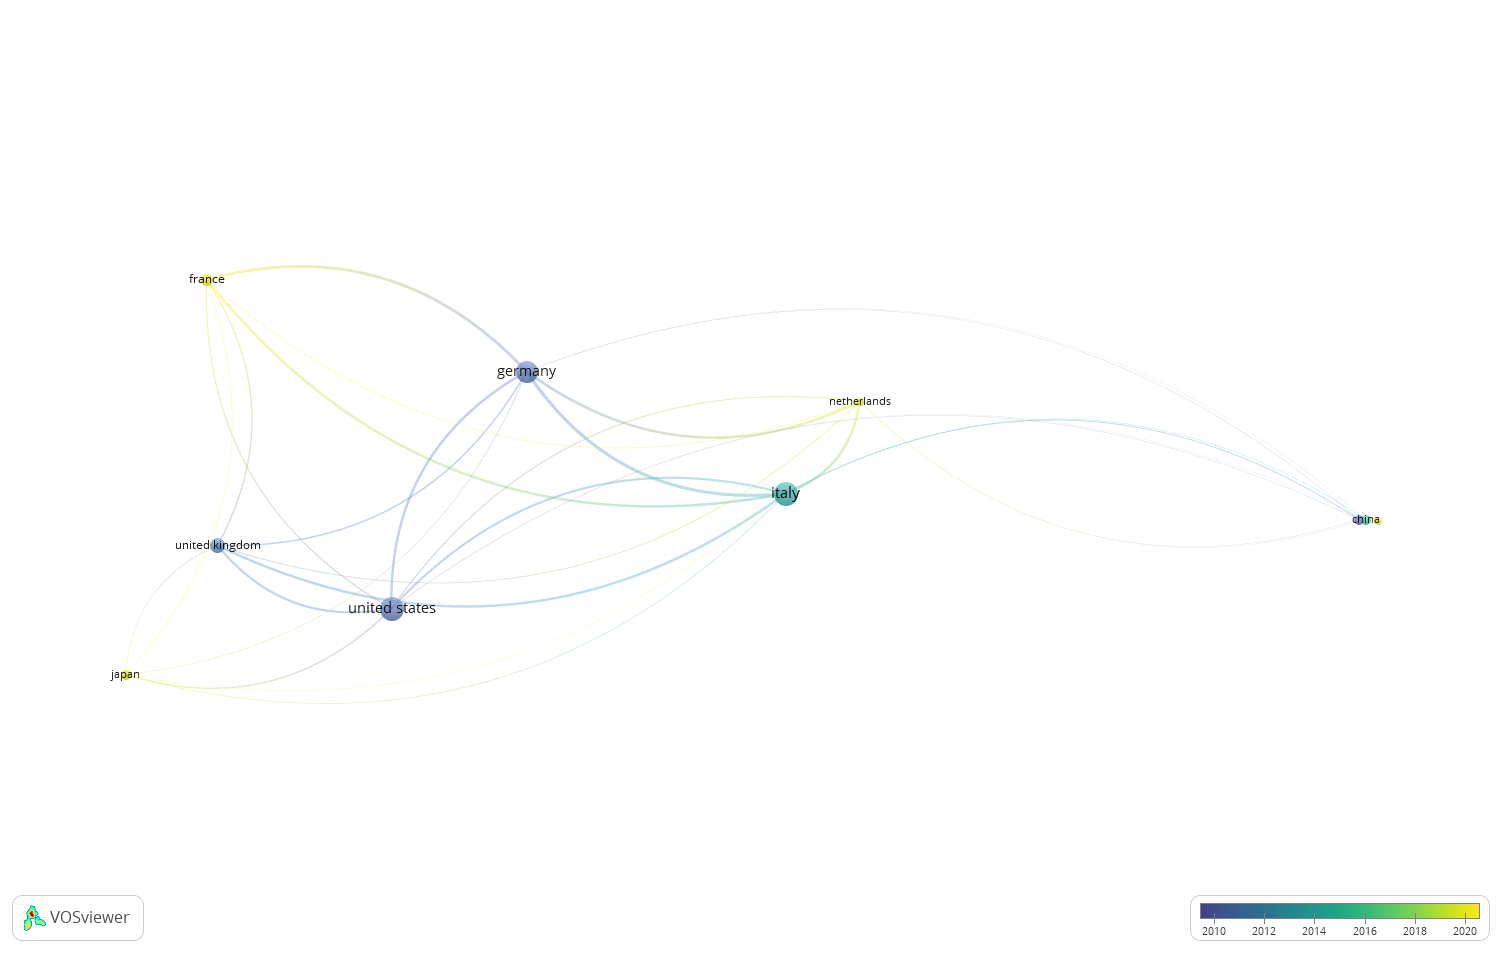
\includegraphics[width=\textwidth]{sfod_b-coupling_countries.png}
\caption{Citation mapping of organizations involved in spacecraft fragmentation and orbital debris research.}
\end{figure}

\subsection{Pybibx}

\textbf{Word cloud visualization}

\begin{figure}[hbt!]
\centering
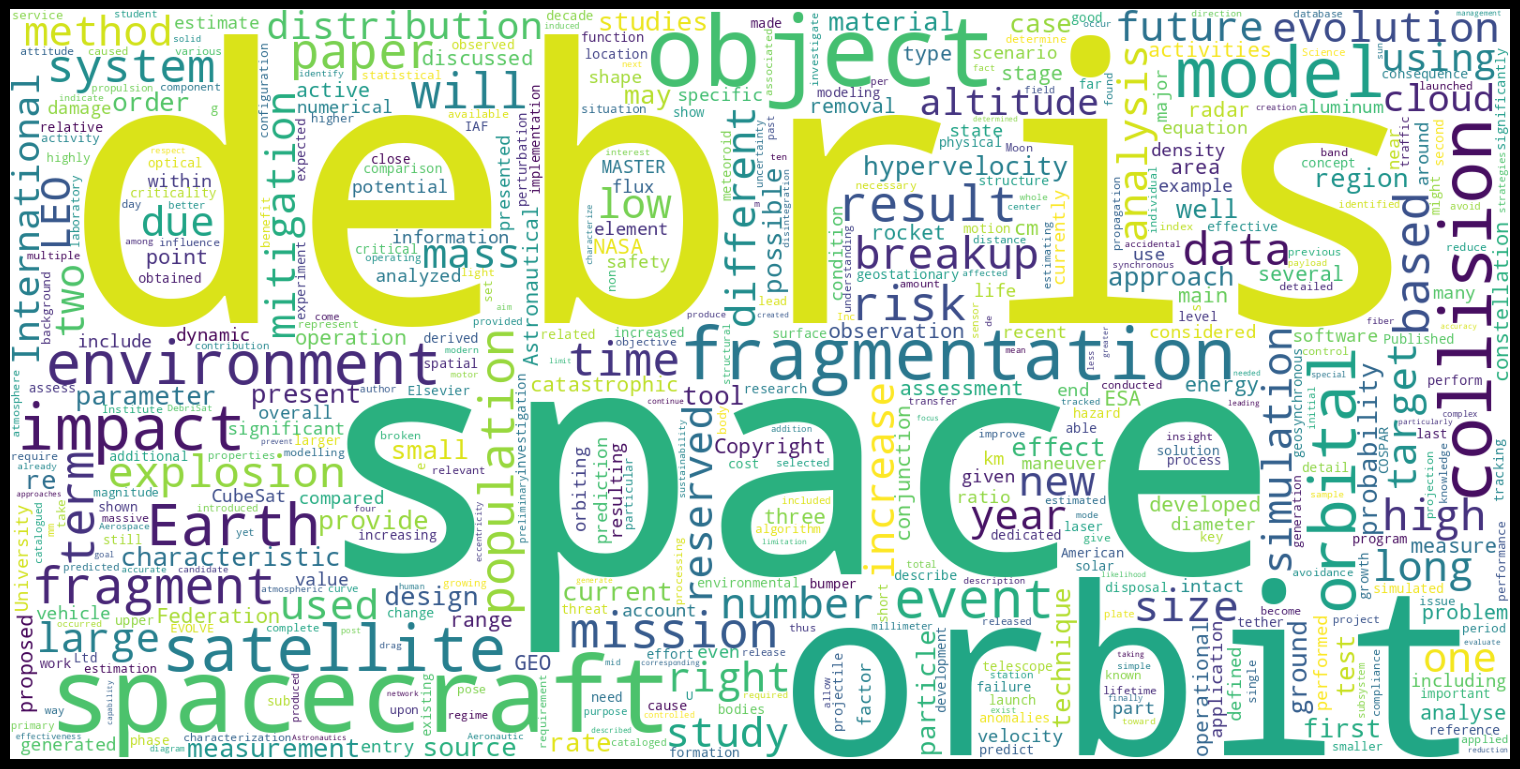
\includegraphics[width=\textwidth]{wc_sfod.png}
\caption{Word cloud visualization.}
\end{figure}

The visualization of cloud clouds of a query on spacecraft fragmentation and orbital debris reveals key themes, terms, and concepts that define focal areas and prevailing concerns in this field. This qualitative analysis offers insight into the main research areas, emerging trends, and focus points within the literature on spacecraft fragmentation and orbital debris. By examining the most frequently occurring terms, several significant aspects of the field can be highlighted.

The dominance of the words "debris" and "space" in the word cloud signifies the centrality of these topics within the literature. This prevalence underscores a research focus on understanding the nature, formation, and management of space debris, particularly in the context of spacecraft fragmentation and its impact on orbital ecosystems. The consistent attention to these topics reflects the urgency of addressing the hazards posed by debris accumulation in space, which has become a critical issue for the safety and sustainability of orbital operations.

The prominence of terms like "orbit" and "collision" indicates the critical issues at the heart of space debris studies. These terms suggest that much of the research revolves around examining the behavior and distribution of debris across different orbital regions and analyzing the mechanics and risks of potential collisions between debris and operational spacecraft. Collision avoidance is evidently a major area of concern, as such incidents pose serious risks to the safety of space operations and the integrity of valuable space assets.

Terms like "modeling," "simulation," and "analysis" feature prominently, suggesting a strong reliance on computational tools in the field. These terms indicate that researchers are using mathematical and physical models to simulate debris creation, movement, and potential collisions, which are essential for assessing risks and developing mitigation strategies. The use of such models highlights the technical rigor required to understand debris dynamics and predict scenarios, providing a foundation for both short-term risk assessments and long-term sustainability planning.

The presence of words like "fragmentation," "explosion," and "impact" points to a specific interest in the mechanisms that generate debris. Researchers appear to be particularly focused on understanding the outcomes of fragmentation events—such as collisions and explosions—that lead to significant debris proliferation. By studying the physics behind these events, scholars aim to model debris formation processes and assess the likelihood of future fragmentation events contributing to the overall debris environment.

Terms like "environment," "risk," and "impact" reveal an ongoing concern for the environmental implications of space debris. Research in this area likely evaluates the potential threats debris poses to current and future space operations, as well as its impact on the broader orbital ecosystem. This aligns with a growing global concern regarding the long-term viability of high-demand orbits, especially in Low Earth Orbit (LEO) and Geostationary Orbit (GEO), which are crucial for both scientific and commercial activities.

The words "population" and "growth" suggest that researchers are examining the increasing quantity of space debris over time, likely analyzing trends and forecasting future scenarios. These studies are crucial for developing strategies to control debris proliferation and avoid a potential cascade effect, commonly known as the Kessler Syndrome, which could render certain orbits unusable. This focus on population growth indicates a proactive approach to managing debris and ensuring the sustainable use of space.

Finally, technical terms like "altitude," "velocity," and "diameter" point to an interest in the physical characteristics of debris. Parameters such as orbital altitude, relative velocity, and size distribution are essential for modeling debris behavior and understanding interactions with other objects in space. Such factors are critical for accurate simulations and for formulating effective mitigation measures.

This kind of analysis sheds light on the research trends and focal points in spacecraft fragmentation and orbital debris studies. The frequent appearance of terms related to risk, environment, and population growth underscores the field's commitment to orbital sustainability. Emphasis on modeling and simulation reflects the reliance on computational tools for predicting debris dynamics and testing mitigation strategies. Furthermore, the attention to collision avoidance, risk assessment, and fragmentation events highlights the technical and safety challenges involved in managing debris. The field’s forward-looking approach, as evidenced by terms like growth and future, shows an awareness of the long-term implications of debris accumulation. This analysis reveals a comprehensive and multifaceted research agenda, merging technical rigor with environmental stewardship and risk management to address the urgent need for sustainable space operations.

\textbf{Evolution}

\begin{figure}[hbt!]
\centering
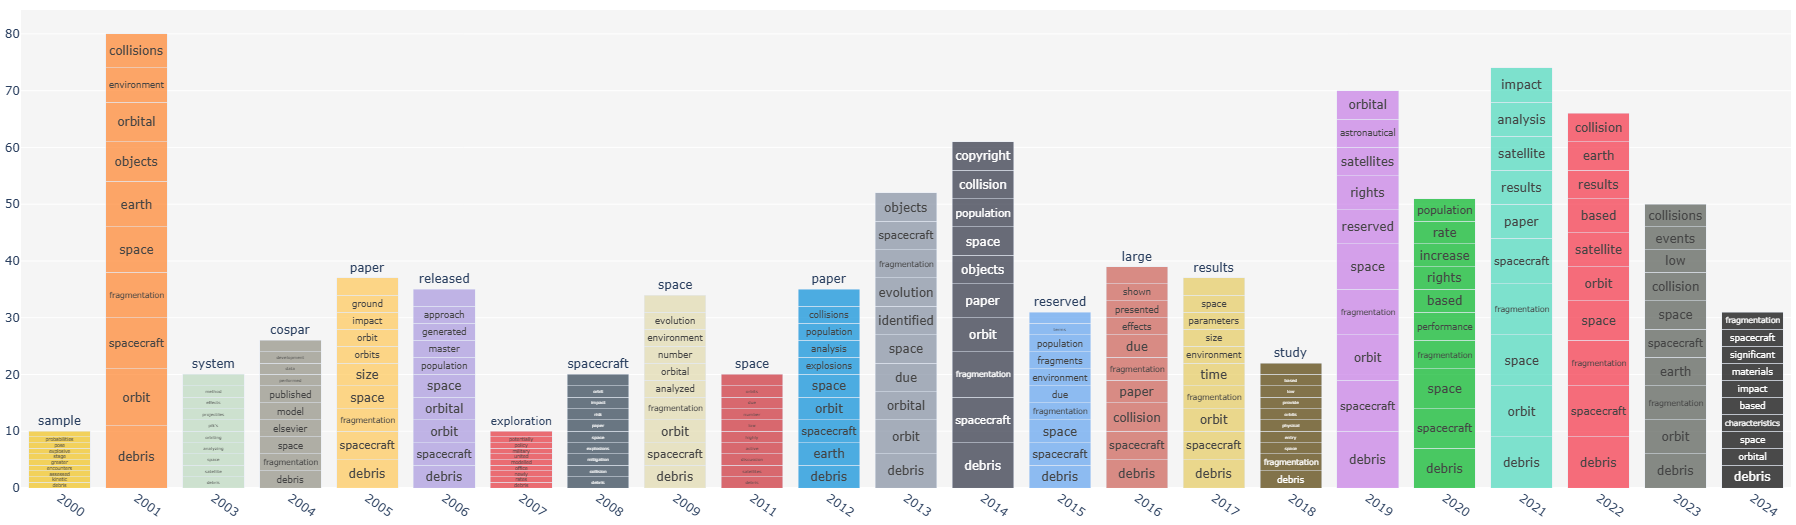
\includegraphics[width=\textwidth]{year_evolution_sfod.png}
\caption{Temporal evolution of key topics in spacecraft fragmentation and orbital debris research.}
\end{figure}

The temporal evolution of key topics in spacecraft fragmentation and orbital debris research reveals a progression from early awareness of collision risks to a sophisticated focus on predictive modeling and detailed analysis of debris characteristics. Initially, the field centered on understanding the fundamental hazards associated with collisions in space and their environmental impact around Earth. This foundational phase laid the groundwork for subsequent research, highlighting the immediate threats posed by fragmentation events and the potential for cascading debris proliferation. The early focus on terms like "collisions," "environment," and "space" underscores a primary concern with the risk of collision-driven debris accumulation and its implications for the orbital environment.

As the field matured, the focus expanded to include the development of systematic modeling tools and databases. Researchers began formalizing approaches for cataloging and studying debris, as reflected by the emergence of terms such as "system" and "generated." This phase marked a critical transition from exploratory studies to structured analyses, supported by databases and modeling frameworks capable of tracking debris and analyzing fragmentation events. This structured approach allowed researchers to better understand the mechanisms of debris generation, track its evolution, and establish frameworks for managing the risks associated with spacecraft fragmentation.

By the mid-2010s, research efforts had shifted towards a comprehensive analysis of debris population growth and long-term orbital sustainability. Keywords such as "population," "evolution," and "analysis" highlight a growing interest in predictive models capable of forecasting the future state of the debris environment. This phase reflects an increased awareness of the cumulative nature of debris in Low Earth Orbit (LEO) and the potential for Kessler Syndrome a scenario in which collisions between debris fragments lead to an uncontrollable cascade of new fragments. Researchers focused on understanding the trajectory of debris population growth and the risks it posed to both current and future missions, resulting in models designed to predict the long-term stability of orbital regions.~\cite{kessler_collision_1978}

In recent years, there has been a heightened focus on the specific risks associated with collision events and the effects of fragmentation on operational satellites. Terms like "collision," "impact," and "satellite" suggest an emphasis on assessing the technical implications of debris for satellite safety and mission sustainability. This phase of research has been characterized by a deeper investigation into the impact of fragmentation events on spacecraft integrity and functionality, alongside the development of collision avoidance and risk mitigation strategies. As the complexity of debris analysis has grown, researchers have refined their models to provide more accurate and actionable insights into debris avoidance and risk reduction for active satellites.

The latest research trends indicate an increasing concern with the material and structural characteristics of debris fragments, as seen in the emergence of terms like "events," "materials," and "characteristics." This focus reflects a shift towards a granular understanding of debris properties, with researchers investigating how different materials and fragment shapes affect debris behavior in orbit. Such insights are crucial for improving debris tracking capabilities, developing more effective mitigation strategies, and informing the design of future spacecraft. By understanding the physical and material properties of debris, researchers aim to enhance prediction models, facilitate more efficient debris removal, and mitigate the risks associated with fragmentation events.

Overall, the evolution of this field demonstrates a shift from broad risk assessment to a highly detailed and specialized analysis of debris dynamics. Early studies laid the groundwork by raising awareness of the collision risks in space, while later research introduced systematic tools for data collection and analysis. The development of predictive models for population growth and the emphasis on material-specific properties highlight a maturing field that is increasingly equipped with the knowledge and tools to manage and mitigate the complex challenges of space debris. The insights gained from recent studies will be instrumental in shaping policies, technological solutions, and operational practices aimed at ensuring the long-term sustainability of orbital environments.

\textbf{Network of Researchers}

\begin{figure}[hbt!]
\centering
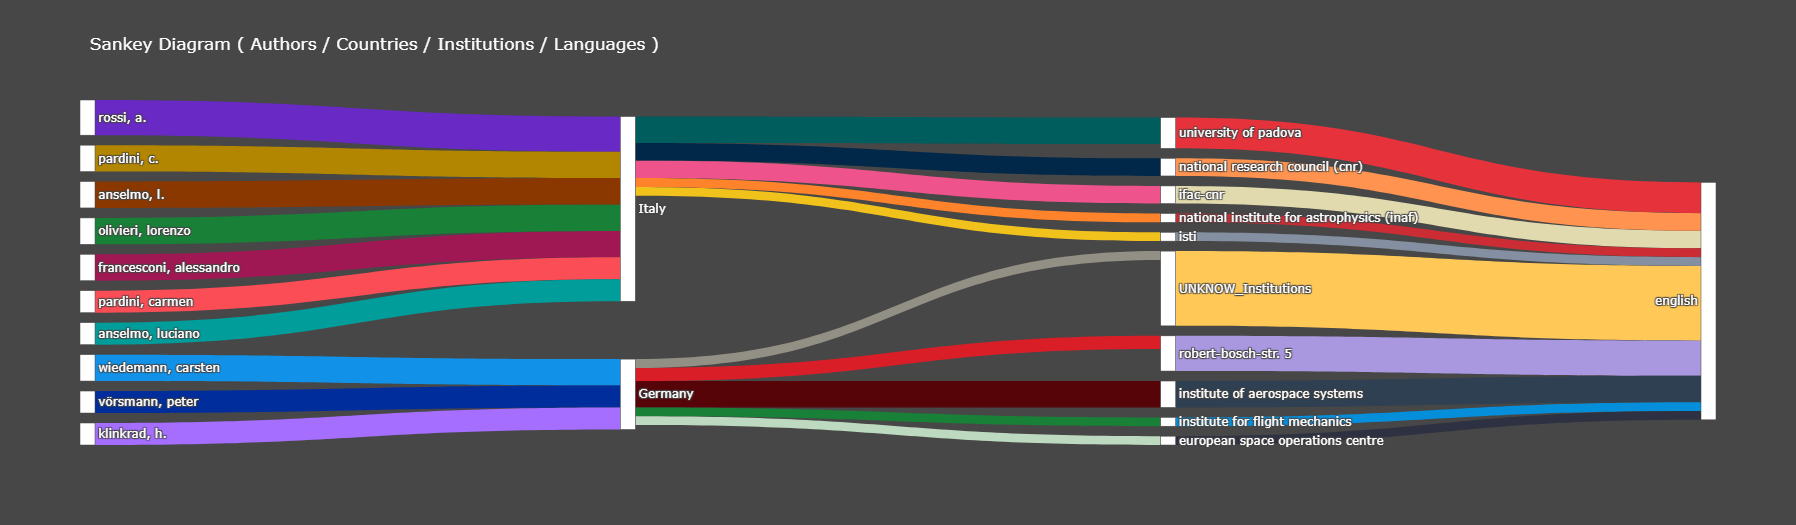
\includegraphics[width=\textwidth]{sankey_sfod.png}
\caption{Sankey diagram illustrating the network of researchers, countries, institutions, and languages in the study of spacecraft fragmentation and orbital debris.}
\end{figure}

The Sankey diagram illustrating the network of researchers, countries, institutions, and languages in the study of spacecraft fragmentation and orbital debris reveals several important insights regarding the field's scholarly composition and its primary contributors. The data shows a strong concentration of research activity originating from Italy and Germany, with notable authors like A. Rossi, C. Pardini, and L. Anselmo linked to Italian institutions such as the University of Padova, the National Research Council (CNR), and other research-focused organizations like IFAC-CNR and the National Institute for Astrophysics (INAF). This prominence of Italian institutions reflects Italy’s substantial role in advancing the study of space debris, underscoring a national commitment to understanding and mitigating the risks posed by fragmentation in Earth’s orbital environment.

Similarly, Germany’s contribution is evident through the works of authors such as Carsten Wiedemann, Peter Vörsmann, and H. Klinkrad, who are affiliated with research organizations and operational centers such as the Institute of Aerospace Systems, the Institute for Flight Mechanics, and the European Space Operations Centre. Germany’s active involvement highlights its technological and research capabilities, particularly in operational aspects of debris tracking, collision avoidance, and space environment monitoring. The collaborative links among authors and institutions within these two nations reflect an environment of concentrated expertise that likely promotes rapid advancements and innovations in debris analysis methodologies.

The diagram also indicates the language predominance in this research field, with English serving as the primary language for communication. This linguistic consistency not only facilitates international collaboration but also underscores the global relevance of the topic, as the language choice ensures accessibility and broader dissemination of research findings to the international scientific community. The recurring presence of English as the primary language strengthens the field’s cohesion by enabling seamless knowledge transfer across borders, contributing to a globally aligned approach to space debris issues.

Another notable aspect of the diagram is the significant role of interdisciplinary and multi-institutional collaborations. The connectivity between various institutions within Italy and Germany implies a cooperative research environment, where knowledge is shared across institutional boundaries to address the complex challenges associated with space debris. This interdisciplinary approach is vital in a field that requires diverse expertise in fields such as astrophysics, aerospace engineering, and orbital mechanics. By drawing upon varied institutional resources and expert perspectives, these collaborative networks support the development of robust and comprehensive solutions to spacecraft fragmentation and debris mitigation. The diagram highlights the leadership roles that Italy and Germany play in the domain of spacecraft fragmentation and orbital debris research, with Italian and German institutions contributing significantly to the field's knowledge base. The reliance on English as the primary language facilitates international engagement and the dissemination of critical findings. The multi-institutional collaborations observed in these countries demonstrate an interdisciplinary approach that enhances the field’s resilience against the complex technical challenges posed by debris accumulation. This collective research effort lays a foundation for informed policy decisions and technical advancements, contributing to the long-term sustainability of the orbital environment.

\textbf{Authors' productivity}

\begin{figure}[hbt!]
\centering
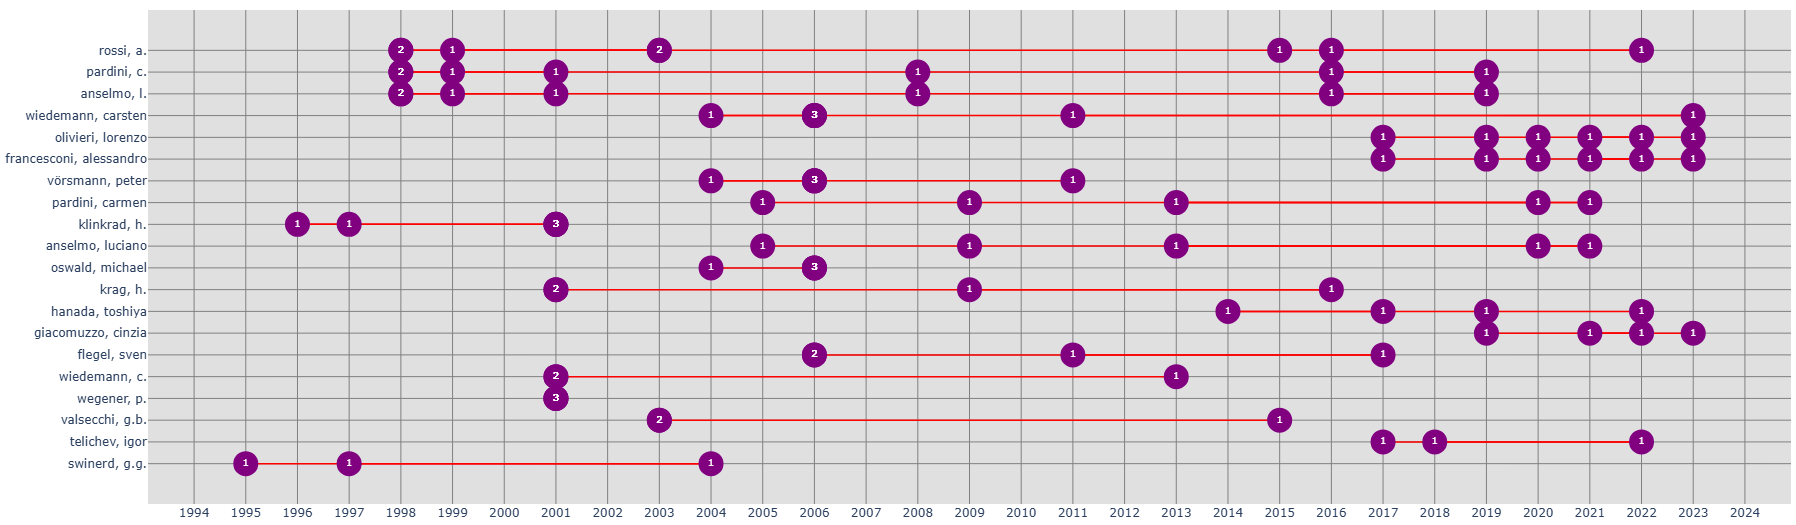
\includegraphics[width=\textwidth]{authors_productivity_sfod.png}
\caption{Visualization of author productivity based on a Scopus query related to spacecraft fragmentation and orbital debris.}
\end{figure}

The analysis of author productivity based on a Scopus query related to spacecraft fragmentation and orbital debris highlights key trends in research output and contributions within this field. The graph illustrates the temporal distribution of publications by various authors, shedding light on both the foundational contributors and those who have made recent impacts. Notably, certain authors, such as David B. Spencer, exhibit a prolonged period of consistent research activity, indicating sustained involvement and potentially a deep expertise in the area. This long-term commitment by some authors may have contributed significantly to foundational knowledge and the development of comprehensive models and theories within spacecraft fragmentation and orbital debris.

The increased clustering of publications by certain authors in recent years reflects a growing research interest and concern in the field. Authors like Tetsuo Yasaka, Hugh G. Lewis, and Roberto Armellin have shown a notable concentration of publications, especially post-2010, suggesting a response to the increasing urgency surrounding orbital debris management. This rise in activity correlates with heightened awareness of space sustainability and the potential hazards posed by an ever-growing debris population in key orbits. As space activities become more frequent and expansive, the concentration of research in recent years signals the scientific community's acknowledgment of the pressing need to address debris accumulation and collision risks in Earth’s orbits.

The graph also indicates that a few authors, such as Francesco Topputo and Eliseo P. Vergara, have contributed intermittently over the years, implying that their contributions might be more specialized or sporadic, likely addressing specific aspects of the spacecraft fragmentation or orbital debris topic. These intermittent contributions could indicate research that targets particular incidents or breakthroughs rather than continuous investigation, highlighting the diversity of research approaches within the field. Some authors may focus on periodic advancements or respond to particular incidents or challenges that arise over time, contributing to the body of knowledge in a more episodic manner.

Moreover, the steady influx of new authors from 2010 onward signifies that spacecraft fragmentation and orbital debris have attracted fresh interest, likely due to emerging technologies, international regulatory focus, and new space initiatives. This new wave of researchers contributes to the expansion of knowledge and innovation, providing fresh perspectives on managing and mitigating space debris. The influx of researchers reflects the interdisciplinary nature of the field, requiring input from various domains including aerospace engineering, environmental science, and computational modeling. This influx may lead to a wider range of methodologies and a more comprehensive approach to tackling the debris problem, encompassing technical solutions as well as policy and management strategies.

\textbf{Colaboration between countries}

\begin{figure}[hbt!]
\centering
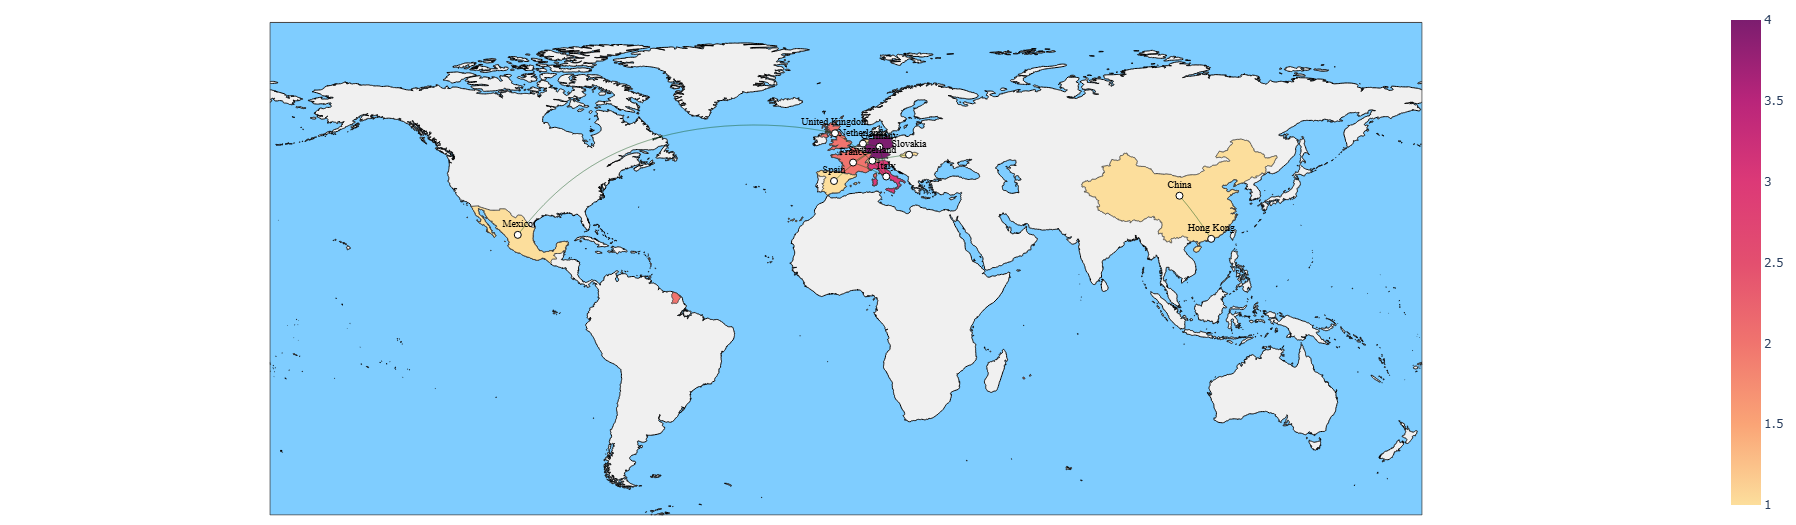
\includegraphics[width=\textwidth]{colab_countries_sfod.png}
\caption{Colaboration between countries in the space debris and fragmentation research.}
\end{figure}

The map illustrating international collaboration in spacecraft fragmentation and orbital debris research highlights notable patterns of cooperation among countries across different continents. Europe stands out as a primary hub of activity, with several countries like the United Kingdom, Germany, Spain, and Italy showing substantial contributions and a strong interconnected network. This close collaboration among European countries may be driven by shared concerns about the sustainability of space activities and the need for collective policies within the European Union and affiliated institutions. The presence of multiple space agencies and research institutions within Europe facilitates cooperative research initiatives, which are crucial for addressing the complex and globally impactful challenges associated with orbital debris.

In addition to Europe, the map indicates significant involvement from countries in North America, particularly the United States and Mexico. The United States, as a leading spacefaring nation with extensive resources allocated to space exploration and satellite deployment, plays a pivotal role in advancing research and development in orbital debris mitigation and space traffic management. Collaborative efforts between the United States and other countries, such as those in Europe, demonstrate a recognition of the global nature of orbital debris issues and an acknowledgment of the need for shared responsibility in maintaining space safety and sustainability.

Asia, represented notably by China and Hong Kong, also appears as an emerging contributor to research in spacecraft fragmentation and orbital debris. China’s increasing engagement in this field aligns with its growing space ambitions and investments in satellite and crewed missions, highlighting a proactive stance in understanding and managing debris created from its space activities. This engagement is essential given China’s extensive activity in low Earth orbit, which is one of the most heavily trafficked and debris-populated regions in space. Collaboration with international counterparts can aid in standardizing debris management practices and aligning with global mitigation frameworks.

Overall, the map underscores a geographically diverse yet concentrated network of countries actively participating in spacecraft fragmentation and orbital debris research. The strong interconnectedness of European countries, alongside active contributions from North America and emerging involvement from Asia, emphasizes the collective and collaborative effort required to tackle the complex issue of space debris. The visualization illustrates that while certain regions dominate in productivity and partnerships, the field is inherently global in scope, with research benefiting from cross-border knowledge exchange and joint initiatives. This international collaboration is critical, as effective debris mitigation and long-term space sustainability demand comprehensive and globally harmonized approaches that transcend national boundaries. The combined efforts of these countries reinforce the urgency and global commitment to addressing the growing challenges posed by space debris, ensuring safer and more sustainable access to outer space for future generations.

\subsection{Litmaps.}

The use of Litmaps in research has emerged as an effective approach for enhancing the process of discovering, analyzing, and visualizing connections between scientific publications. Litmaps allow researchers to create an interactive network of literature, highlighting the relationships between articles, authors, and research themes over time. This tool is particularly advantageous for areas of research that are rapidly evolving or interdisciplinary, as it enables researchers to identify emerging trends, influential papers, and potential gaps in knowledge. By mapping the scholarly landscape, Litmaps facilitate a more comprehensive understanding of how different ideas and studies converge, evolve, or branch out over time. The dynamic visualization that Litmaps provide goes beyond static citation charts, allowing for a more intuitive exploration of how a particular topic has developed and where it might be heading.

When Litmaps was applied to space debris and orbital fragmentation research, the benefits were significant. Space debris is an increasingly critical topic due to its implications for satellite operations, space exploration, and the overall sustainability of activities in low Earth orbit (LEO) and beyond. Given this field's highly technical and multifaceted nature, the ability to map out the relationships between studies on spacecraft fragmentation, debris propagation models, and mitigation strategies is invaluable. Here. the queries described above were combined to create a broad picture of the papers involved as a whole.

The Litmaps visualization of the research on spacecraft fragmentation, orbital debris, and propagators provides an insightful analysis of the field’s evolution and its influential works. The map shows connections between 464 publications, highlighting how the research community has built upon foundational works over time. The horizontal axis indicates the timeline of publication (from left to right: older to more recent publications), while the vertical axis indicates the number of citations each paper has received (lower to higher citations).

Analyzing the map from the perspective of recent publications and their impact (measured by citations), it is evident that there are several papers published from 2021 onwards that have garnered considerable attention. Notable recent publications that stand out include those by Jenkins (2021)~\cite{jenkins_strathcube_2021} and Zhou (2022)~\cite{zhang_tde-based_2022}. These papers are positioned further right on the map, indicating their recent publication dates, and higher up, suggesting they have accumulated significant citations within a relatively short time. This reflects their immediate influence and importance in the ongoing discourse surrounding space debris and orbit propagation models.

The map also reveals seminal works that continue to be highly cited, even years after publication. The papers by Liou (2006, 2009)~\cite{liou_collision_2006}~\cite{liou_controlling_2010} and Rein (2011, 2015)~\cite{rein_rebound_2012}~\cite{rein_whfast_2015} appear prominently, showing their status as the cornerstone of research in the field. Liou’s work is particularly influential, contributing foundational knowledge on space debris mitigation and long-term orbital sustainability. Rein’s publications have also had a substantial impact, particularly regarding computational methods and propagators for modeling n-body dynamics and orbital debris.

Further analysis shows that foundational papers published before 2010 by Kessler (1978, 1991)~\cite{kessler_environment_1985} remain influential, serving as the basis for subsequent research and being frequently cited by newer publications. Kessler’s early work on the cascading effect of space debris, known as the "Kessler Syndrome," continues to inform both theoretical studies and policy discussions.

Recent works showing promising influence include those by Olivieri (2023)~\cite{olivieri_analysis_2023}, Pisanu (2023)~\cite{pisanu_recent_2021}, and Lamb (2018)~\cite{h_lamb_space_2018}, positioned in the lower right quadrant, suggesting that they are recent yet accumulating citations at a growing pace. These papers may be addressing innovative approaches to space debris modeling or the application of new computational techniques such as symplectic propagators in simulating complex orbital scenarios.

\begin{figure}[hbt!]
\centering
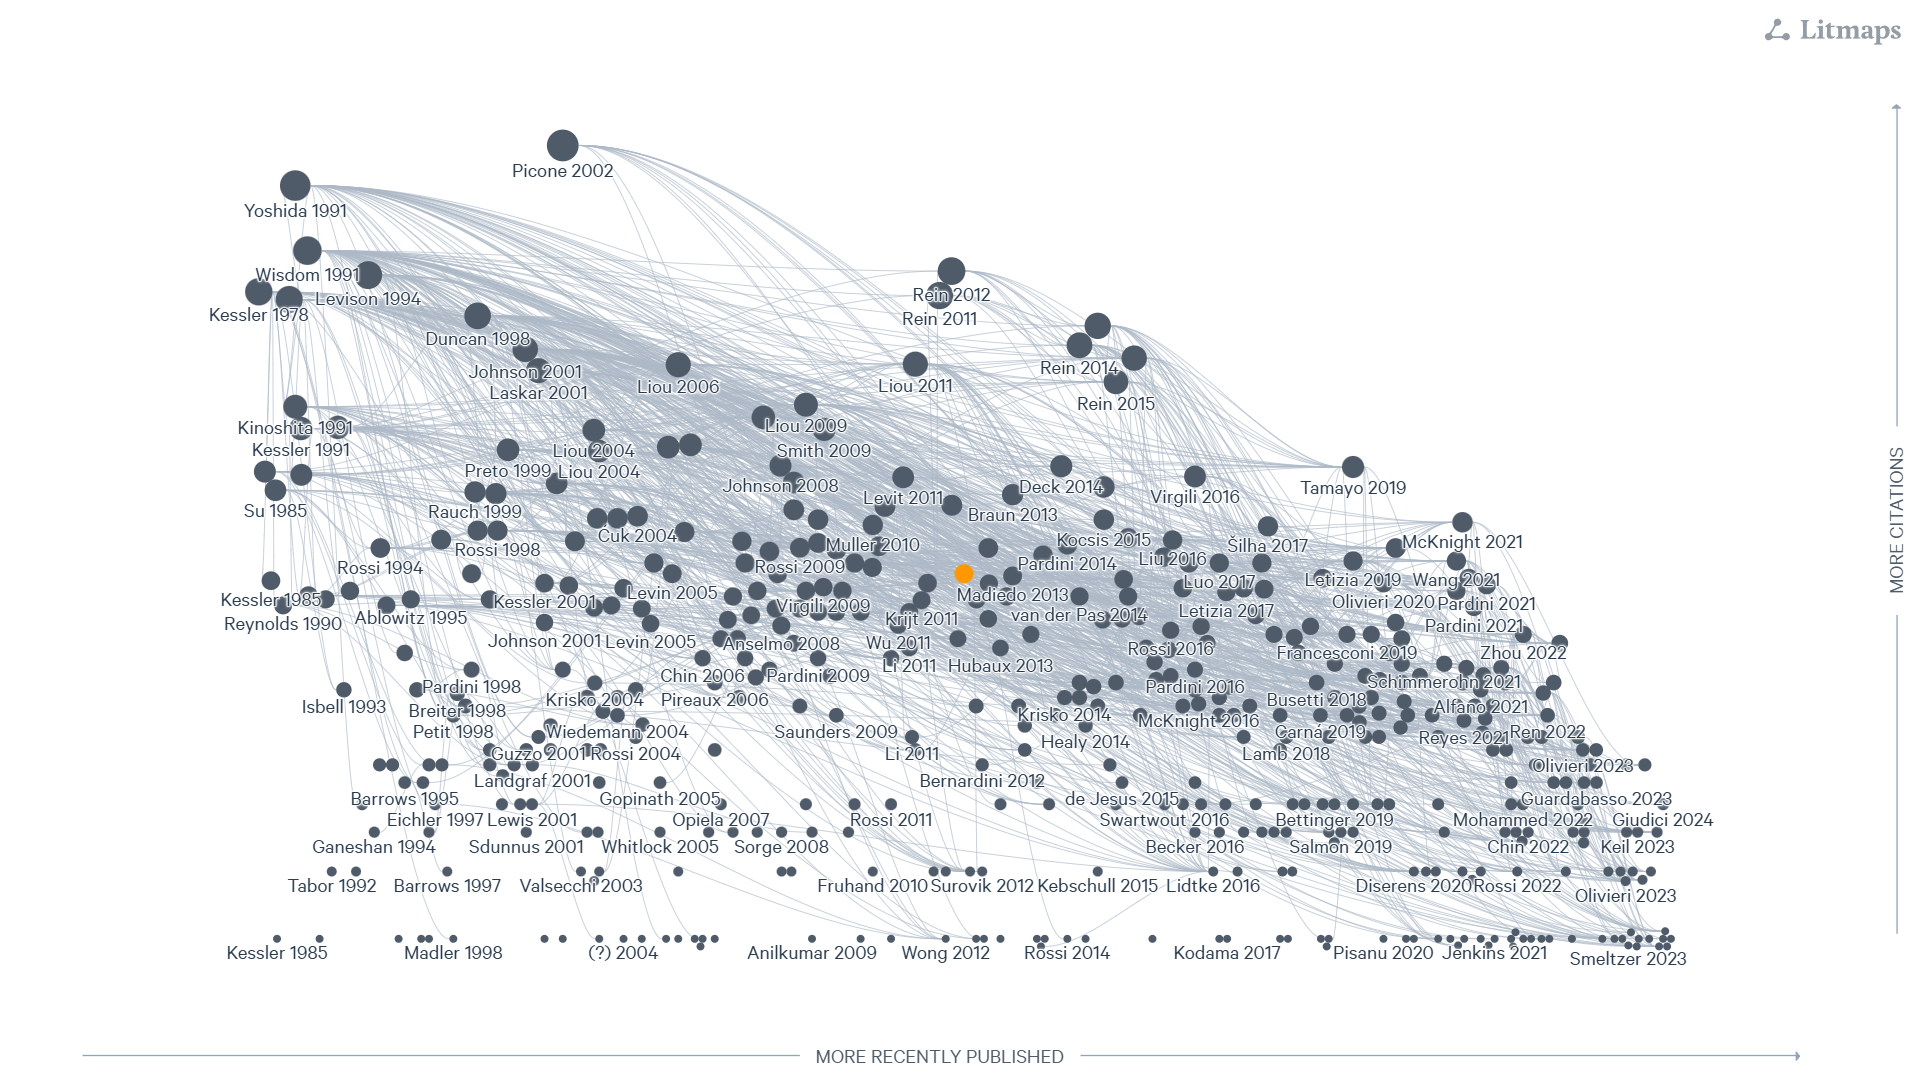
\includegraphics[width=\textwidth]{Litmaps_whole.png}
\caption{Litmaps image for the date and citation of the analyzed papers related to the literature review.}
\end{figure}

\section{Discussion}

The bibliometric analysis reveals several key insights that are crucial for understanding the landscape of research on space debris fragmentation and multibody orbit propagation. 

\subsection{Key Authors and Influential Publications.}
The analysis identifies several thought leaders in the field, including authors such as Francesca Letizia and J.-C. Liou, whose works are frequently cited. Influential publications, such as the NASA Standard Breakup Model and studies on the Kessler Syndrome, contribute significantly to the understanding of fragmentation dynamics and debris population modelling. These works provide foundational knowledge that informs my research objectives, particularly in developing more accurate models to predict debris behavior.

A comprehensive analysis of the Kessler Syndrome is essential, as its implications extend beyond theoretical models to real-world scenarios where cascading collisions could render critical orbital regions unusable, jeopardizing both current and future space missions.

\subsection{Collaboration Patterns.}
The analysis highlights dominant collaboration patterns, indicating a trend toward international partnerships between research groups. Notable collaborations are evident between institutions in Europe and the United States, particularly in studies focusing on debris mitigation strategies and orbital dynamics. This collaborative environment fosters the exchange of ideas and methodologies, which is essential to advance research in this complex field.

The role of international collaboration and policy frameworks, such as those established by the Inter-Agency Space Debris Coordination Committee (IADC)~\cite{noauthor_iadc_nodate}, is crucial to develop cohesive strategies to manage space debris effectively and ensure the sustainability of space operations.

\subsection{Research Gaps and Opportunities.}
Despite the wealth of literature, the analysis uncovers several research gaps, particularly in the modeling of smaller debris fragments and their long-term impact on orbital sustainability. Areas such as the integration of AI in debris tracking and the development of real-time monitoring systems remain under-researched. This research could address these gaps by focusing on innovative modeling techniques and exploring the application of machine learning to improve the accuracy of debris prediction.

\subsection{Trends and Evolution.}
Emerging trends in aerospace engineering indicate a growing focus on space sustainability and the application of AI in aerospace systems. The increasing number of satellites and the associated risks of collisions highlight the need for effective debris management strategies. This trend aligns with my research objectives, which aim to contribute to the development of sustainable practices in space operations.

Recent advances in radar and optical tracking systems, as well as the development of machine learning algorithms for debris prediction, have significantly improved our ability to monitor the space environment. Evaluating the effectiveness of these technologies, in conjunction with current mitigation strategies, will offer a more comprehensive understanding of the challenges facing the field.

\section{Conclusions}

The bibliometric analysis conducted across various documents has yielded several key insights that are highly relevant to the PhD research on space debris fragmentation and its implications for orbital sustainability. The analysis revealed trends in the frequency of fragmentation events, the characteristics of debris generated, and the effectiveness of current mitigation strategies. In particular, the findings indicate a significant increase in the number of cataloged objects due to intentional and accidental collisions, with catastrophic events contributing substantially to the debris population ~\cite{pardini_review_2014}. This underscores the urgent need for improved debris tracking and modeling to improve space situational awareness.

\subsection{Research Implications}
\subsubsection{Practical Implications}
The insights gained from the analysis highlight the need for robust debris mitigation strategies and the development of advanced tracking systems. Understanding the dynamics of fragmentation events and their contributions to the debris environment will inform the design of more effective post-mission disposal (PMD) strategies and collision avoidance protocols. This is particularly relevant for my research, as it emphasizes the importance of integrating real-time data from space surveillance systems to improve the accuracy of debris models.

\subsubsection{Theoretical Implications}
The analysis also points to gaps in the theoretical frameworks used to model debris generation and propagation. The findings suggest that existing models may not adequately account for the complexities of fragmentation dynamics, particularly in relation to the size and velocity distributions of debris fragments ~\cite{mains_impact_2022}. This indicates a need for the development of more sophisticated models that incorporate empirical data from recent fragmentation events, which will be a focus of my research.

\subsection{Future Directions}
Future research can build on these findings by addressing the identified gaps in understanding fragmentation processes and their long-term effects on the orbital environment. Specifically, there is a need for:

\begin{enumerate}
    \item Enhanced Modeling Techniques: Future studies should focus on refining fragmentation models to better predict the size and distribution of debris generated from various types of collision. This could involve the integration of machine learning techniques to analyze historical fragmentation data and improve predictive accuracy ~\cite{giudici_density-based_2024}.
    \item Longitudinal studies: Conducting longitudinal studies on the evolution of debris populations over time will provide valuable insight into the effectiveness of current mitigation strategies and the potential for catastrophic collisions. This aligns with the findings that indicate a need for ongoing assessment of the debris environment ~\cite{petit_impact_2016}.
    \item Interdisciplinary approaches: Future research should adopt interdisciplinary approaches that combine information from engineering, environmental science, and policy studies to develop comprehensive strategies for debris mitigation. This could involve collaboration with space agencies and industry stakeholders to implement best practices in satellite design and operation ~\cite{olivieri_large_2020}.
\end{enumerate}

By addressing these future directions, the research will contribute to a more nuanced understanding of space debris dynamics and inform the development of effective strategies to ensure the sustainability of orbital regions. The insights gained from the bibliometric analysis will be instrumental in refining the research questions, objectives, and overall approach, ensuring that the work is relevant and impactful in the field of space debris management.

\bibliography{articles}
\bibliographystyle{IEEEtran} %apalike

\end{document}
